\documentclass[11pt]{article}
\usepackage{minted, tikz, blindtext}
\usepackage{amsfonts, amssymb, amsmath, float}
\usepackage{enumerate, esint, nicefrac, algorithm2e}
\parindent 0px
\date{November 2, 2023}
\title{CS301 :: Midterm 2}
\author{Ryan Magdaleno\\80/80 Score}

% Helpful ::
% \line(1,0){358px}
\begin{document}
\maketitle

%%%%%%%%%%%%%%%%%%%%%%%%%%%%%%%%%%%%%%%%%%%%%%%%%%%%%%%%%%%%%%%%%%%%%%%%%%%%%%%%%%%%%%%%%

\textbf{Problem 1. Multiple Choice}

\vspace{5px}\textbf{Solution ::} 
\begin{enumerate}[a)]
\item Which of the following means that a grammar is ambiguous? \\
There is a string with multiple parse trees in the grammar.
\item Which of the following is not a member of the 7-tuple for a TM? \\
$F =$ The set of final states.
\item T/F. Deterministic and Non-deterministic Pushdown Automata decided the same
same set of languages.
False.
\item Which is a valid rule in a right-linear single-step grammar with $a\in\Sigma$
and $A, S\in V$? \\
$S\rightarrow aA$.
\item T/F. All finite languages are context-free. \\ True.
\item Which of the following languages is not context-free? \\
$\{0^a1^b2^c \,|\, a\le b, b\le c\}$
\item Context-Free languages are not closed which of the following operations? \\
Intersection ($\cap$).
\item Which of the following rules is not context-free? \\
$bSb\rightarrow bab$.
\item Which is not a possible outcome of computation in a Turing Machine? \\
Contradiction.
\item T/F. All Turing-recognizable languages are Turing-decidable. \\
False.
\end{enumerate}
\pagebreak

%%%%%%%%%%%%%%%%%%%%%%%%%%%%%%%%%%%%%%%%%%%%%%%%%%%%%%%%%%%%%%%%%%%%%%%%%%%%%%%%%%%%%%%%%

\textbf{Problem 2. Short Answer}
\begin{enumerate}[a)]
\item
What are the elements of the 6-tuple for a PDA? \\
\vspace{5px}\textbf{Solution ::}
\begin{align*}
    Q &= \text{Set of states.} \\
    \Sigma &= \text{Alphabet set of input characters.} \\
    \Gamma &= \text{Alphabet set of stack characters.} \\
    \delta &= \text{Transition function:} \\
    &\hspace{16px}Q\times (\Sigma\cup\{\epsilon\})\times (\Gamma\cup\{\epsilon\})
    \longrightarrow P(Q\times (\Gamma\cup\{\epsilon\})) \\
    q_0 &= \text{Starting state.} \\
    &\hspace{16px}q_0\in Q \\
    F &= \text{Set of final states} \\
    &\hspace{16px}F\subseteq Q
\end{align*}
\line(1,0){343px}

\item
Given CFGs $G_1 = (V_1, \Sigma, R_1, S_1)$ and $G_2 = (V_2, \Sigma ,R_2, S_2)$
that decide languages $L_1$ and $L_2$ respectively, describe how to construct
a CFG which accepts the concatenation of $L_1$ and $L_2$. You may either
describe how to construct the CFG that accepts their concatenation, or give
the 4-tuple for the CFG that accepts their concatenation. \\
\vspace{5px}\textbf{Solution ::}
\begin{align*}
    S_0 &= \text{New starting state.} \\
    V &= V_1\cup V_2\cup \{S_0\} \\
    \Sigma &= \Sigma_1 = \Sigma_2 \\
    R &= R_1 \cup R_2 \cup \{S_0\longrightarrow S_1S_2\} \\
    S &= S_0
\end{align*}
\line(1,0){343px}

\item
Give an example of a language that is context-free but not regular. \\
\vspace{5px}\textbf{Solution ::}
$$L = \{0^n1^n \,|\, n\ge 0\}$$
\end{enumerate}
\pagebreak

%%%%%%%%%%%%%%%%%%%%%%%%%%%%%%%%%%%%%%%%%%%%%%%%%%%%%%%%%%%%%%%%%%%%%%%%%%%%%%%%%%%%%%%%%

\textbf{Problem 3. Context-Free Grammars} \\
Give a Context-free grammar for the following language $L$. \\
$\Sigma = \{a,b,c,d\}$
$$L = \{a^ib^jc^kd^k \,|\, 0 < i < j, k\ge 1\}$$
\vspace{5px}\textbf{Solution ::}
\begin{align}
    S&\longrightarrow aXbcYd \\
    Y&\longrightarrow\epsilon\,|\, cYd \\
    X&\longrightarrow aXb\,|\, B \\
    B&\longrightarrow bB\,|\, b
\end{align}
\pagebreak

%%%%%%%%%%%%%%%%%%%%%%%%%%%%%%%%%%%%%%%%%%%%%%%%%%%%%%%%%%%%%%%%%%%%%%%%%%%%%%%%%%%%%%%%%

\textbf{Problem 4. PDA Construction} \\
Create the PDA which decided the following language $L$. \\
$\Sigma = \{a,b,c\}$
$$L = \{a^nb^{2n}c^m\,|\,n\ge 0,m\ge 1\}$$
\vspace{5px}\textbf{Solution ::}
\begin{center}
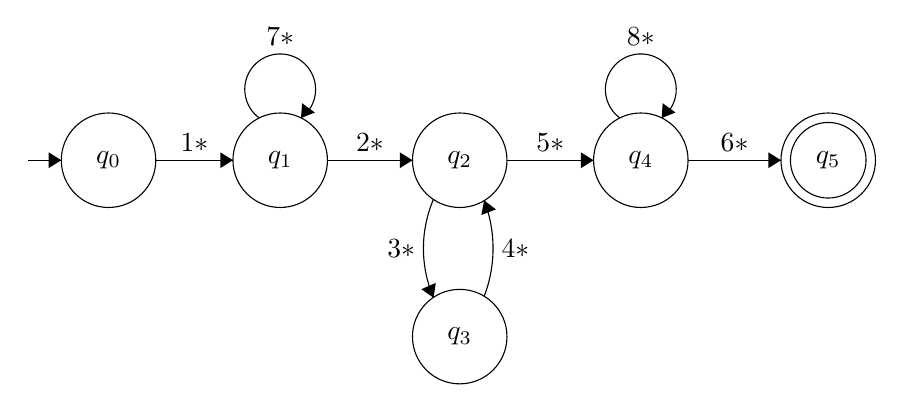
\begin{tikzpicture}[scale=0.2]
\tikzstyle{every node}+=[inner sep=0pt]
\draw [black] (12.4,-20.4) circle (3);
\draw (12.4,-20.4) node {$q_0$};
\draw [black] (23.3,-20.4) circle (3);
\draw (23.3,-20.4) node {$q_1$};
\draw [black] (34.7,-20.4) circle (3);
\draw (34.7,-20.4) node {$q_2$};
\draw [black] (46.2,-20.4) circle (3);
\draw (46.2,-20.4) node {$q_4$};
\draw [black] (58.1,-20.4) circle (3);
\draw (58.1,-20.4) node {$q_5$};
\draw [black] (58.1,-20.4) circle (2.4);
\draw [black] (34.7,-31.6) circle (3);
\draw (34.7,-31.6) node {$q_3$};
\draw [black] (7.3,-20.4) -- (9.4,-20.4);
\fill [black] (9.4,-20.4) -- (8.6,-19.9) -- (8.6,-20.9);
\draw [black] (15.4,-20.4) -- (20.3,-20.4);
\fill [black] (20.3,-20.4) -- (19.5,-19.9) -- (19.5,-20.9);
\draw (17.85,-19.9) node [above] {$1*$};
\draw [black] (26.3,-20.4) -- (31.7,-20.4);
\fill [black] (31.7,-20.4) -- (30.9,-19.9) -- (30.9,-20.9);
\draw (29,-19.9) node [above] {$2*$};
\draw [black] (33.035,-29.126) arc (-156.8696:-203.1304:7.957);
\fill [black] (33.04,-29.13) -- (33.18,-28.19) -- (32.26,-28.59);
\draw (31.9,-26) node [left] {$3*$};
\draw [black] (36.248,-22.951) arc (21.10402:-21.10402:8.467);
\fill [black] (36.25,-22.95) -- (36.07,-23.88) -- (37,-23.52);
\draw (37.32,-26) node [right] {$4*$};
\draw [black] (37.7,-20.4) -- (43.2,-20.4);
\fill [black] (43.2,-20.4) -- (42.4,-19.9) -- (42.4,-20.9);
\draw (40.45,-19.9) node [above] {$5*$};
\draw [black] (49.2,-20.4) -- (55.1,-20.4);
\fill [black] (55.1,-20.4) -- (54.3,-19.9) -- (54.3,-20.9);
\draw (52.15,-19.9) node [above] {$6*$};
\draw [black] (21.977,-17.72) arc (234:-54:2.25);
\draw (23.3,-13.15) node [above] {$7*$};
\fill [black] (24.62,-17.72) -- (25.5,-17.37) -- (24.69,-16.78);
\draw [black] (44.877,-17.72) arc (234:-54:2.25);
\draw (46.2,-13.15) node [above] {$8*$};
\fill [black] (47.52,-17.72) -- (48.4,-17.37) -- (47.59,-16.78);
\end{tikzpicture}
\end{center}
\begin{align*}
    \Gamma &= \{\$, A\} \\
    1* &= \epsilon,\,\epsilon\longrightarrow \$ \\
    2* &= \epsilon,\,\epsilon\longrightarrow\epsilon \\
    3* &= b,\,A\longrightarrow\epsilon \\
    4* &= b,\,\epsilon\longrightarrow\epsilon \\
    5* &= c,\,\epsilon\longrightarrow\epsilon \\
    6* &= \epsilon,\,\$\longrightarrow\epsilon \\
    7* &= a,\,\epsilon\longrightarrow A \\
    8* &= c,\,\epsilon\longrightarrow\epsilon
\end{align*}
\pagebreak

%%%%%%%%%%%%%%%%%%%%%%%%%%%%%%%%%%%%%%%%%%%%%%%%%%%%%%%%%%%%%%%%%%%%%%%%%%%%%%%%%%%%%%%%%

\textbf{Problem 5. Chomsky Normal Form} \\
Convert the following grammar to CNF.
\begin{align*}
    S&\longrightarrow xAy\,|\, AB \\
    A&\longrightarrow AB\,|\, xA \\
    B&\longrightarrow yB\,|\,\epsilon
\end{align*}
\vspace{5px}\textbf{Solution ::} \\
\textbf{START ::}
\begin{align}
    S_0 &\longrightarrow S \\
    S &\longrightarrow xAy\,|\, AB \\
    A&\longrightarrow AB\,|\, xA \\
    B&\longrightarrow yB \,|\,\epsilon
\end{align}
\textbf{BIN ::}
\begin{align}
    S_0&\longrightarrow S \\
    S&\longrightarrow xS_1 \,|\, AB \\
    S_1&\longrightarrow Ay \\
    A&\longrightarrow AB\,|\, xA \\
    B&\longrightarrow yB \,|\,\epsilon
\end{align}
\textbf{DEL ::}
\begin{align}
    S_0&\longrightarrow S \\
    S&\longrightarrow xS_1 \,|\,AB\,|\, A \\
    S_1&\longrightarrow Ay \\
    A&\longrightarrow AB\,|\, A\,|\, xA \\
    B &\longrightarrow yB \,|\, y
\end{align}
\textbf{UNIT ::}
\begin{align}
    S_0&\longrightarrow XS_1\,|\, AB\,|\, xA \\
    S&\longrightarrow XS_1\,|\,AB\,|\,xA \\
    S_1&\longrightarrow Ay \\
    A&\longrightarrow AB \,|\, xA\\
    B&\longrightarrow yB\,|\,y
\end{align}

\pagebreak
\textbf{TERM ::}
\begin{align}
    S_0&\longrightarrow U_0S_1\,|\, AB\,|\, U_0A \\
    S&\longrightarrow U_0S_1\,|\,AB\,|\,U_0A \\
    S_1&\longrightarrow AU_1 \\
    A&\longrightarrow AB\,|\, U_0A \\
    B&\longrightarrow U_1B\,|\, Y \\
    U_0&\longrightarrow x \\
    U_1&\longrightarrow y
\end{align}
\pagebreak

%%%%%%%%%%%%%%%%%%%%%%%%%%%%%%%%%%%%%%%%%%%%%%%%%%%%%%%%%%%%%%%%%%%%%%%%%%%%%%%%%%%%%%%%%

\textbf{Problem 6. Non-Context-Free Proof} \\
Prove that the following language $L$ is not context-free.
$$L=\{0^i1^j2^i\,|\,j<i\}$$
\vspace{5px}\textbf{Solution ::}

Suppose for the sake of contradiction, that $L$ is context-free. Then, by \\definition,
there must be a CFG $G$ with pumping length $p$ that generates it. \\
Let $s = 0^{p+1}1^p2^{p+1}$ \\
By the pumping length, $s$ can be partitioned into $u,v,x,y,z$ such that
$|vxy|\le p$ and $|vy| \ge 1$. We proceed on cases for $v$ and $y$:
\begin{enumerate}[\hspace{5px}-]
\item 
$v/y$ are contained within the 1s. If we were to set $vxy$ to $k$ 1s for some
$k \ge 1$ such that $|vxy|\le p$. By the pumping lemma if we pump up let's
say $i=10$, we would generate $\ge 10$ 1s which makes our total 1s atleast
$p+10$ which makes our inequality $j<i$ false. This new string is $\notin L$,
a contradiction.

\item
$v/y$ are contained within only the 0s or 2s. If we were to set $vxy$ to $k$ 0s
(or 2s), for some $k\ge 1$ such that $|vxy|\le p$. By the pumping lemma if we
pump up or down i, i.e. $i\neq 1$, $i\ge 0$, the \# of 0s would not match
the $p+1$ 2s or vice versa. Similarily this occurs when $vxy$ is contained
within 0s and 1s or 1s and 2s, a contradiction.
\end{enumerate}
All cases result in a contradiction of the pumping lemma. \\
$\therefore L$ is not context-free.


\end{document}